\newpage
\chapter{Diskussion}

Dette projekt valgte vi at dele op i en række delmål. Delmålene var delt op i grupperne Basics, Advanced, Brikker, Helhedsindtryk og Hardware. Basics var det der skulle til for at få et fungerende spil og de efterfølgende mål har skullet opfylde vores ønsker om at lave et realistisk spil med godt gameplay. Ud fra disse delmål, samt det ekstra mål at man skulle kunne få powerups i spillet, lavede vi tidsplanen vist på Figur \ref{fig:tidsplan2}, øverst. Som det kan ses nederst på samme figur, tog implementeringen af brikkerne dog væsentlig længere tid end forventet og det gjorde at vi ikke nåede vores mål om at lave powerups. En anden forskel på vores oprindelige tidsplan og hvad vi rent faktisk gjorde, var at vi startede tidligere på at dokumentere projektet og dette er dermed blevet gjort løbende. Undervejs i forløbet valgte vi at lave ASCII-art til spillet. Vi valgte at gøre dette da vi havde et spil hvor fysikken fungerede tilfredsstillende. Med ASCII-arten vil vi gerne give spillet en stemning af et old-school, gennemført arkadespil.

\begin{figure}[h!]
\centering
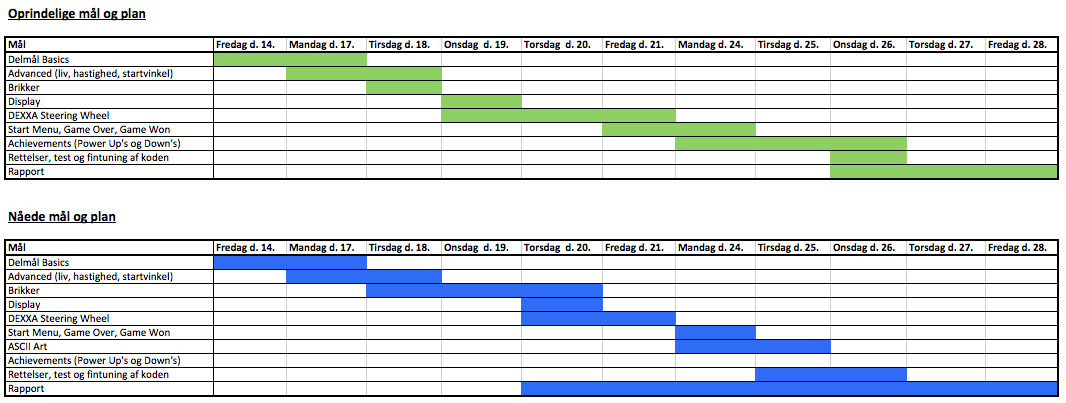
\includegraphics[scale=0.4]{figs/Tidsplan2.png}
\caption{Øverst: Tidsplan over de forskellige delmål og hvornår de skulle være færdige. Nederst: Hvad vi rent faktisk lavede og hvornår}
\label{fig:tidsplan2}
\end{figure}

Forsinkelserne i projektet som kan ses på Figur \ref{fig:tidsplan2}skyldtes primært at vi, sammen med de avancerede delmål, valgte at gøre bolden større. Da vi skiftede til terminalen putty i stedet for HyperTerminal og fik mulighed for at køre terminalen i fuldskærm valgte vi at lave bolden $4\times2$ karakterer. Dette gjorde, at bolden kunne ramme flere brikker af gangen, og briklogikken blev af den grund meget kompleks, se flowchartet på Figur \ref{fig:brickFlow} og  Appendix \nameref{reflexball}. En yderligere udfordring var, at bolden bevægede sig to karakterer af gangen i x-retningen på skærmen. Der kunne derfor komme en stor del af bolden ind i brikkerne, hvilket også vanskeliggjorde, at fastslå, hvordan brikken var blevet ramt af bolden. \\ 
En stor del af arbejdet med brikkerne bestod af debugging og rettelser i koden. For at teste briklogikken skrev vi tekst ud på skærmen der fortalte os hvordan vi havde ramt brikkerne, om flagene \texttt{dontDeflectX} og \texttt{dontDeflectY} var blevet sat og om det var detekteret at der var brikker ved siden af og over/under den ramte brik. På den måde kunne vi finde præcis de steder i koden hvor der var problemer med vores logik.\\

Hvis vi skulle have implementeret powerups i spillet kunne det være gjort ved at tjekke om en brik døde hver gang man ramte en brik. Hvis den gjorde det, kunne vi f.eks. lade de sidste tre bit af millis() bestemme om man fik en powerup. Hvis de sidste tre bit gav f.eks. 0 kunne man få en powerup. På den måde ville det være tilfældigt om man fik en powerup, man ville have 1/8 sandsynlighed for at det skete. \\
Den store udfordring med powerups er dog at implementere en masse forskellige sjove festures de skulle have. En powerup kunne f.eks. give langsom hastighed, flere bolde, bredere striker, større/mindre bold, blinkende eller usynlig striker, blinkende level, flere brikker, mulighed for  at skyde eller mange andre ting. For at det skulle være en gennemført implementering af powerups skulle vi dog lave flere forskellige funktioner, og dette ville derfor blive et forholdsvis stort arbejde. Vi valgte derfor at fokusere på at lave et gennemført spil hvor der var tænkt over detaljerne. 



Skriv verifikationsafsnit
	Globale variabler
	Problemer med brikker og bold
	Nåede ikke power-ups og power-downs
	Fandt undervejs ud af vi ville inkludere ASCII-Art
	Hvad vi nåede og hvad vi ikke nåede (se tidsplan2.png
	Hvordan vi har testet det hele


